\documentclass[paper,twocolomn]{geophysics}
%\documentclass[manuscript]{geophysics}

%\documentclass[manuscript,endfloat]{geophysics}
\usepackage{amsmath,amssymb,amsfonts,graphicx,subfigure,bm,yfonts,hyperref,cleveref,xcolor}
\usepackage{rotating}
%\usepackage[outdir=./]{epstopdf}

\usepackage{multirow}


%%%%%%%%%                              DEFINITIONS START

\def\cpar{$C_{ij},\rho$ parameterization~}
\def\hpar{h-parameterization~}

\newcommand{\todo}[1]{{\textbf {\color{red} #1}}}
\newcommand{\done}[1]{{\bf {\color{green} #1}}}
\newcommand{\connect}{{\textbf{\color{red} $<-$ Connect $->$ }}}


\def\rmrk#1{{\textbf{[[#1]]}}}
\def\rmrkok#1{}
%\def\eqref#1{\ref{#1}}
\def\eqrf#1{equation~\eqref{eq:#1}}
%\def\eqref#1{equation~\ref{eq:#1}}
\def\eq{equation~}
\def\figref#1{Figure~\ref{fig:#1}}
\def\figrefp#1{(Figure~\ref{fig:#1})}

\def\fref#1{\ref{#1}}

\def\rhoK{\hat{\rho}}
\def\cK{\hat{c}}


%\def\rmrk#1{{[\textcolor[rgb]{0,0,0.8}{#1}]}} % [blue]
%\def\rmrkm#1{{\textbf{[[\textcolor[rgb]{{1.00,0.00,0.00}}{#1}]]}}}
% _____________________________________________________________________________
\def\mainauthor{Vladimir Kazei}
\def\coauthorb{Ekkehart Tessmer}
\def\coauthorc{}%Zedong Wu
\def\coauthora{Tariq Alkhalifah}
% - my definitions==============================================================================================

\def\DP{Diffraction-based radiation 
patterns }
\def\dP{diffraction-based radiation 
patterns }

\def\nt{N}
\newcommand{\Mod}[1]{\ (\mathrm{mod}\ #1)}
\def\dv{\mathbf{d}}
\def\Amat{\mathbb{A}}
\def\Rmat{\mathbb{R}}
\def\Umat{\mathbb{U}}
\def\Smat{\mathbb{S}}
\def\Vmat{\mathbb{V}}
\def\SF{R}
\def\xv{\mathbf{x}}
\def\mv{\mathbf{m}}
%\def\tmul{\otimes}
\def\tmul{}
\def\cv{\mathbf{c}}

\def\sp{\varsigma}
\def\spv{\bm{\sp}}
\def\gp{\xi}
\def\gpv{\bm{\gp}}

\newcommand{\nmz}[1]{\mathbf{\bar{\text{$#1$}}}}
%\def\nmz#1{\mathbf{\bar #1}}

\def\Uv{\mathbf{U}}
\def\kv{\mathbf{k}}
\def\sv{\mathbf{s}}
\def\svn{\mathbf{\bar{\sv}}}
\def\Sv{\mathbf{S}}
\def\Gv{\mathbf{G}}
\def\Cv{\mathbf{C}}
\def\ev{\mathbf{e}}
\def\gv{\mathbf{g}}
\def\gvn{\mathbf{\bar{\gv}}}
\def\Av{\mathbf{A}}
\def\Bv{\mathbf{B}}
\def\uv{\mathbf{u}}
\def\rv{\mathbf{r}}
\def\dxv{\Delta \mathbf{x}}
\def\Kv{\mathbf{K}}
\def \cost{ \cos \frac{\theta}{2}}
%\newcommand{\sdot}{\mathbf{\bullet}}

\newcommand{\sdot}{{WI-WS, \delta \mv}}

\newcommand{\inty}{\int\limits_{-\infty}^{+\infty}}
\newcommand{\intyt}{\inty\inty\inty}
\newcommand{\intyV}{\int\limits_{V}}

\def\Rp{\mathcal{R}}
\def\Dp{\mathcal{D}}
\def\Tp{\mathcal{T}}
%\def\Cp{\mathcal{C}}
\def\Sp{\mathcal{S}}

% - Tariq's definitions begin here ==============================================================================
\def\beq{\begin{eqnarray}}
\def\eeq{\end{eqnarray}}

\def\mmbx#1{{\mathbf{#1}}}

\def\phi{\varphi}

\def\Vv{\mmbx{V}}
\def\gammav{\pmb{\gamma}}
\def\epsv{\pmb{\eps}}
\def\deltav{\pmb{\delta}}
\def\etav{\pmb{\eta}}

\def\v{V}
\def\rhov{\pmb{\rho}}
\def\r{\mmbx{r}}
\def\k{\mmbx{k}}

\def\d{\text{d}}
\def\c{\mmbx{c}}
\def\e{\mmbx{e}}
\def\m{\mmbx{m}}
\def\x{\mmbx{x}}
\def\xs{\x_s}
\def\xr{\x_r}
\def\L{\mmbx{L}}
\def\p{\mmbx{p}}
\def\q{\mmbx{q}}

\def\La{{\cal L}}
\def\tf{\tilde{f}}
\def\tA{\tilde{A}}
\def\ttau{\tilde{\tau}}
\def\y{\mmbx{y}}
\def\z{\mmbx{z}}

\def\tm{\tilde{m}}
\def\tr{\tilde{r}}
\def\tw{\tilde{w}}
\def\tv{\tilde{v}}
\def\tp{\tilde{p}}
\def\tq{\tilde{q}}

\def\a{\mmbx{a}}
\def\H{\mmbx{H}}
\def\g{\mmbx{g}}
\def\W{\mmbx{W}}

\def\eps{\varepsilon}

\def\La{{\cal L}}

\def\tlambda{\tilde{\lambda}}
\def\tw{\tilde{w}}

\def\rvn{r_{v_n}}
\def\rvh{r_{v_h}}
\def\rrho{r_\rho}
\def\rdel{r_\delta}
\def\reta{r_\eta}
\def\reps{r_\eps}


\def\Re{{{\cal{R}}_e}}

\newcommand{\pd}[2]{\frac{\partial #1}{\partial #2}}

%==============================================end of Tariq's notation=========================================


%%%%%%%%%								DEFINITIONS END
\newcommand{\mylabel}[1]{\label{#1}}
\newcommand{\myrf}[1]{\ref{#1}}

%%\newcommand{\plot}[3]{
%	\begin{figure}
%		\center
%		\includegraphics[#2]{Fig/#1}
%		\caption{#3}
%		\label{fig:#1}
%	\end{figure}
%}

\newcommand{\aplot}[3]{
	\begin{figure}[htbp!]
		\center
		\includegraphics[#2]{#1}
		\caption{#3}
		\label{fig:#1}
	\end{figure}
}

\newcommand{\twplot}[3]{
	\begin{figure}
		\centering
		\subfigure[]{\includegraphics[width=0.4\columnwidth]{Fig/#1}
			\label{fig:#1}}
		\hspace*{-0.01\columnwidth}
		\subfigure[]{\includegraphics[width=0.55\columnwidth]{Fig/#2}
			\label{fig:#2}}
		\caption{#3}
		%\label{fig:#1}
	\end{figure}
}

\newcommand{\tplot}[4]{
	\begin{figure}
		\centering
		\subfigure[]{\includegraphics[width=0.3\columnwidth]{Fig/#1}
			\label{fig:#1}}
		\vspace*{-0.01\columnwidth}
		\subfigure[]{\includegraphics[width=0.3\columnwidth]{Fig/#2}
			\label{fig:#2}}
		\vspace*{-0.01\columnwidth}
		\subfigure[]{\includegraphics[width=0.3\columnwidth]{Fig/#3}
			\label{fig:#3}}
		\caption{#4}
		\label{fig:#1_#3}\label{fig:#1_Full}
	\end{figure}
}
\newcommand{\tplott}[4]{
	\begin{figure}
		\centering
		\subfigure[]{\includegraphics[width=0.2\columnwidth]{Fig/#1}
			\label{fig:#1}}
		\vspace*{-0.01\columnwidth}
		\subfigure[]{\includegraphics[width=0.4\columnwidth]{Fig/#2}
			\label{fig:#2}}
		\vspace*{-0.01\columnwidth}
		\subfigure[]{\includegraphics[width=0.3\columnwidth]{Fig/#3}
			\label{fig:#3}}
		\caption{#4}
		\label{fig:#1_#3}\label{fig:#1_Full}
	\end{figure}
}
\newcommand{\tplotv}[4]{
	\begin{figure}
		\centering
		\subfigure[]{\includegraphics[width=0.49\columnwidth]{Fig/#1}
			\label{fig:#1}}
		\vspace*{-0.01\columnwidth}
		\subfigure[]{\includegraphics[width=0.49\columnwidth]{Fig/#2}
			\label{fig:#2}}
		\vspace*{-0.01\columnwidth}
		\subfigure[]{\includegraphics[width=0.49\columnwidth]{Fig/#3}
			\label{fig:#3}}
		\caption{#4}
		\label{fig:#1_#3}\label{fig:#1_Full}
	\end{figure}
}

\newcommand{\ffplot}[5]{
	\begin{figure}
		\centering
		\subfigure[]{\includegraphics[height=0.47\columnwidth]{Fig/#1}
			\label{fig:#1}}
		\hspace*{0.01\columnwidth}
		\subfigure[]{\includegraphics[height=0.47\columnwidth]{Fig/#2}
			\label{fig:#2}}
		\hspace*{-0.01\columnwidth}
		\subfigure[]{\includegraphics[height=0.47\columnwidth]{Fig/#3}
			\label{fig:#3}}
		\hspace*{0.01\columnwidth}
		\subfigure[]{\includegraphics[height=0.47\columnwidth]{Fig/#4}
			\label{fig:#4}}
		\caption{#5}
		\label{fig:#1:#4}\label{fig:#1_Full}
		\vspace*{-0.03\columnwidth}
	\end{figure}
}

\newcommand{\fplot}[5]{
	\begin{figure}
		\centering
		\subfigure[]{\includegraphics[height=0.27\columnwidth]{Fig/#1}
			\label{fig:#1}}
		\hspace*{0.01\columnwidth}
		\subfigure[]{\includegraphics[height=0.27\columnwidth]{Fig/#2}
			\label{fig:#2}}
		\hspace*{-0.01\columnwidth}
		\subfigure[]{\includegraphics[height=0.27\columnwidth]{Fig/#3}
			\label{fig:#3}}
		\hspace*{0.01\columnwidth}
		\subfigure[]{\includegraphics[height=0.27\columnwidth]{Fig/#4}
			\label{fig:#4}}
		\caption{#5}
		\label{fig:#1:#4}\label{fig:#1_Full}
		\vspace*{-0.03\columnwidth}
	\end{figure}
}

\newcommand{\splot}[7]{
	\begin{figure}
		\centering
		\subfigure[]{\includegraphics[height=0.27\columnwidth]{Fig/#1}
			\label{fig:#1}}
		\hspace*{0.01\columnwidth}
		\subfigure[]{\includegraphics[height=0.27\columnwidth]{Fig/#2}
			\label{fig:#2}}
		\hspace*{-0.01\columnwidth}
		\subfigure[]{\includegraphics[height=0.27\columnwidth]{Fig/#3}
			\label{fig:#3}}
		\hspace*{0.01\columnwidth}
		\subfigure[]{\includegraphics[height=0.27\columnwidth]{Fig/#4}
			\label{fig:#4}}
		\subfigure[]{\includegraphics[height=0.27\columnwidth]{Fig/#5}
			\label{fig:#5}}
		\subfigure[]{\includegraphics[height=0.27\columnwidth]{Fig/#6}
			\label{fig:#6}}
		\caption{#7}
		\label{fig:#1:#6}\label{fig:#1_Full}
		\vspace*{-0.03\columnwidth}
	\end{figure}
}

\newcommand{\fiPlot}[6]{
	\begin{figure}
		\centering
		\subfigure[]{\includegraphics[width=0.31\columnwidth]{Fig/#1}
			\label{fig:#1}}
		\hspace*{-0.01\columnwidth}
		\subfigure[]{\includegraphics[width=0.31\columnwidth]{Fig/#2}
			\label{fig:#2}}
		\hspace*{-0.01\columnwidth}
		\subfigure[]{\includegraphics[width=0.31\columnwidth]{Fig/#3}
			\label{fig:#3}}
		\hspace*{-0.01\columnwidth}
		\subfigure[]{\includegraphics[width=0.33\columnwidth]{Fig/#4}
			\label{fig:#4}}
		\subfigure[]{\includegraphics[width=0.33\columnwidth]{Fig/#5}
			\label{fig:#5}}
		\caption{#6}
		\label{fig:#1:#5}\label{fig:#1_Full}
	\end{figure}
}

\newcommand{\dplot}[3]{
	\begin{figure}
		\centering
		\subfigure[]{\includegraphics[height=0.45\columnwidth]{Fig/#1}
			\label{fig:#1}}
		\hspace*{-0.01\columnwidth}
		\subfigure[]{\includegraphics[height=0.45\columnwidth]{Fig/#2}
			\label{fig:#2}}
		\vspace*{-0.01\columnwidth}
		\caption{#3}
		\label{fig:#1:#2}\label{fig:#1_Full}
	\end{figure}
}

\newcommand{\ddplot}[3]{
	\begin{figure}
		\centering
		\subfigure[]{\includegraphics[width=0.7\columnwidth]{Fig/#1}
			\label{fig:#1}}
		\hspace*{-0.01\columnwidth}
		\subfigure[]{\includegraphics[width=0.99\columnwidth]{Fig/#2}
			\label{fig:#2}}
		\vspace*{-0.01\columnwidth}
		\caption{#3}
		\label{fig:#1_#2}\label{fig:#1_Full}
	\end{figure}
}

\def\ewidth{0.4}


\newcommand{\eplot}[9]{
	\begin{figure}
		\centering
		\subfigure[]{\includegraphics[width=\ewidth\columnwidth]{Fig/#1}
			\label{fig:#1}}
		\hspace*{-0.01\columnwidth}
		\subfigure[]{\includegraphics[width=\ewidth\columnwidth]{Fig/#2}
			\label{fig:#2}}
		\hspace*{-0.01\columnwidth}
		\subfigure[]{\includegraphics[width=\ewidth\columnwidth]{Fig/#3}
			\label{fig:#3}}
		\hspace*{-0.01\columnwidth}
		\subfigure[]{\includegraphics[width=\ewidth\columnwidth]{Fig/#4}
			\label{fig:#4}}
		\hspace*{-0.01\columnwidth}
		\subfigure[]{\includegraphics[width=\ewidth\columnwidth]{Fig/#5}
			\label{fig:#5}}
		\hspace*{-0.01\columnwidth}
		\subfigure[]{\includegraphics[width=\ewidth\columnwidth]{Fig/#6}
			\label{fig:#6}}
		\hspace*{-0.01\columnwidth}
		\subfigure[]{\includegraphics[width=\ewidth\columnwidth]{Fig/#7}
			\label{fig:#7}}
		\hspace*{-0.01\columnwidth}
		\subfigure[]{\includegraphics[width=\ewidth\columnwidth]{Fig/#8}
			\label{fig:#8}}
		\caption{#9}
		%\label{fig:#1}
	\end{figure}
}


\graphicspath{{./Fig/}}

\begin{document}

\title{Mapping full seismic waveforms to vertical velocity profiles by deep learning}

\renewcommand{\thefootnote}{\fnsymbol{footnote}} 

\author{Vladimir Kazei, Oleg Ovcharenko, Pavel Plotnitskii, Daniel Peter, Xiangliang~Zhang \& Tariq Alkhalifah}
\address{
King Abdullah University of Science and Technology (KAUST), Thuwal, 23955-6900, Saudi Arabia \\
vladimir.kazei@kaust.edu.sa, oleg.ovcharenko@kaust.edu.sa, pavel.plotnitskii@kaust.edu.sa, \\
daniel.peter@kaust.edu.sa, xiangliang.zhang@kaust.edu.sa, tariq.alkhalifah@kaust.edu.sa}


\footer{submitted to Geophysics}
\lefthead{Kazei et al.}
\righthead{\emph{Velocity model building by deep learning}}

\maketitle

\begin{abstract}
	Building realistic and reliable models of the subsurface is the primary goal of seismic imaging.
	Full-waveform inversion (FWI) allows us to incorporate realistic physical descriptions of the Earth’s subsurface through modeling to deliver high-resolution estimates of the subsurface parameters.
	However, FWI is a local optimization technique and hence requires a good initial model to start. Also, FWI relies on iterative modeling of full-wavefields; therefore, it is computationally expensive.
	Here we construct an ensemble of convolutional neural networks (CNNs) to build velocity models directly from the data.
	CNNs are trained to map the seismic data directly into velocity logs. This allows us to integrate well data into the inversion and to simplify the mapping by using the regularity of active seismic acquisition. 
	The presented approach uses gathers of neighboring common midpoints (CMPs) for the estimation of a vertical velocity log to accommodate larger dips relative to single CMP gathers. At the same time, we still benefit from the regularity of sampling in seismic exploration. 
	Once the network is trained on a particular data set, data sets with similar acquisition parameters can be inverted much faster than with conventional FWI.
\end{abstract}
%\end{document}

%\section{abstract}



	




%% figure naming convention:
%(train/test)_(prefix(single-CMP/multiCMP))_{folder(for train: ""=x1,x2,x3:marmvel1D, marmvel1D_distorted,marmvel,overthrust1D,overthrust2D)}_{inverted/true/X_scaled}


%\newpage
\section{Introduction}
% what is the problem? FWI needs better starting model
% why FWI?
Seismic imaging and inversion suffer from fundamental ambiguities, such as lack of ultra-low frequencies in the data and ultra-long offsets. This lack of critical data results in the well-known gap in the intermediate wavenumber illumination of the subsurface models \citep{claerbout1985, mora1989, sirgue2004, alkhalifahFullmodelWavenumberInversion2016, kazei2016, kazei2018, yao2019extraction}. In most cases, this gap is significant and causes difficulties when building smooth background models. The low frequencies can in principle be acquired together in a long-offset acquisition \citep[e.g.][]{fons2013}, yet that is a very expensive solution to the problem of insufficient middle wavenumber information.

% solutions?
%\todo{Rephrase the paragraph} %FWI turned out to be so powerful and the problem of the lack of low frequencies in common exploration surveys is so challenging that possible solutions have been under development for decades.

Numerous modifications have been proposed to make full-waveform inversion (FWI) work without low-frequency data. %We will split them into three generations.
% misfits
Conventionally, the lack of low-wavenumber information is addressed by changing the data misfit functionals in FWI \citep[e.g.][]{luo1991wave, bozdag2011, choi2012, leeuwen2013, sun2019robust}.
Introducing advanced model regularization techniques, such as total variation or more generally Sobolev space norms \citep[e.g.][]{esserTotalvariationRegularizationStrategies2016, kazeiSaltbodyInversionMinimum2017, kalita2019regularized, skopintseva2019regularization} into the inversion is another approach that improves low wavenumber coverage in FWI.
% gradients
Gradient filtering and conditioning \citep{ravaut2004multiscale, alkhalifahFullmodelWavenumberInversion2016, kazei2016, ovcharenko2018, ruan2018global} is easier to tune and achieves similar results in FWI. All the methods listed above are computationally intensive and require parameter tuning.

% deep learning
Alternatively, low wavenumber information can, to some extent, be inferred directly from the data in the form of artificial low frequencies \citep{ovcharenkoNeuralNetworkBased2017, ovcharenkoLowFrequencyDataExtrapolation2018, ovcharenko2019deep, jin2018learn, sunLowFrequencyExtrapolation2018, sun2019extrapolated, kazei2019realistically}. Low-dimensional models \citep[e.g.][]{polo2018, wu2018inversionnet} can be directly inferred from the data. Moreover, for models similar to the training data set (e.g. generated with the same model generator), deep learning can provide resolution comparable to conventional FWI \citep{farris2018tomography, araya2020fast}. A step forward in terms of the estimated model complexity and generalization is, however, not as easy; the labels are images and they are rather big. The beauty of deep learning applications in seismic inversion and velocity model building is that, while training can be very computationally intensive, the application of the trained neural network is computationally very cheap. With the growth of computational power, acoustic FWI has become a prominent tool in high-resolution velocity model building \citep[e.g.][]{warner2013}. On the other hand, anisotropic elastic FWI is still not widely applied due to the large computational cost and large null-spaces associated with multiparameter inversion \citep{kohn2015,kazei2018,kazei2019scattering, podgornovaResolutionVTIAnisotropy2018}. Deep learning applications to the multiparameter inversion of seismic data \citep{ivanov2017traveltime, dramsch2019deep, zhang2019regularized} can help address the issue of the null space.
The ability to apply the trained neural network quickly can also help to analyze the uncertainty in FWI coming from the initial model.



% what shall we change?
The full-waveform-based methods listed above usually do not exploit the regularity of active seismic-exploration sampling. Deep learning can infer mapping for seismic data into the subsurface at a given location, and then reapply it at another location. Most of the attempts are made to infer models as a whole \citep{richardson2018seismic, wu2018inversionnet, zhang2018velocitygan, yang2019deep, oye2019velocity, farris2018tomography, araya2019deep, araya2020fast}. Here we propose utilizing only relevant data from neighboring CMP gathers to estimate a single vertical velocity log at a given location. This setup effectively reduces the dimensionality of the target model space and simplifies the learning procedure. We also expect the trained neural network to be versatile for applications to other models, since it corresponds to estimating a log, not a full model.
%Other available information in the form of well logs is also not normally utilized. 
%We will show how to build realistic models for deep learning training from these logs. 
% and 
%We believe that the computational efficiency of training can be improved by exploiting the regularity of conventional seismic sampling.

% how can we utilize the regularity of seismic sampling?
The paper is organized as follows. First, we discuss the regularity of sampling and seismic data relevance.
%
Then, we construct synthetic subsurface models for training purposes by using elastic and affine transforms of an existing model.
%
After that, we numerically explore a single-CMP versus a multiple-CMP training of a CNN and its application on the constructed synthetic models.
%
%Later we show that single CMP approach fails for geological models that vary laterally and we fix the problem with a multiCMP setup.
%
Later, we apply our ``multiCMP" CNN ensemble on realistic velocity models (Marmousi II and SEAM Phase I). 
%
In the last numerical test, we explore a combination of the multiCMP CNN with FWI on the Overthrust model. 

Finally, we discuss the implications of further applications of the method and draw conclusions.



%Our solution belongs to the last class of methods too.
%
%
%
%One particular feature of exploration seismic data that is underutilized in FWI and and waveform based velocity model building tools is that the data are typically regularly sampled. Tis means that the inversion in different locations may be revealing very different subsurface structures but the data are aquired in the same way. The most straightforward way to acknowledge the data feature is through 1D assumption. \cite{roth1994} mapped shot gathers into 1D velocity profiles and \cite{zheng2019} mapped CMP gathers into velocity logs. It would be unfair to expect more complicated structures to be revealed from single CMP gathers. Here we show the limitations of single CMP mapping and propose an extension to multiple CMP gathers, that allows us to accomodate later variations in the model.
%
%
%
%
%
%
%
%
%
%
%Without prior assumptions inversion is very ill-posed and non-unique.
%
%% how is it typically handled?
%
%
%
%
%Typical way of tackling the non-uniqueness is by introducing a regularization term into inversion. With deep learning it is also possible, but there is another opportunity to just design models that are realistic (satisfy the prior assumptions) for training of the network. 
%
% 
%Deep learning is not new to seismic inversion \citep{roth1994}, yet it emerged main stream in the very past years. Several recent applications claim to yield good results, yet most of the models revealed with the help of deep learning are relatively simple and unrealistic. Here we show that neural networks can be applied to obtain models with fine features and realistic structures.
%
%this brings efforts low frequency extrapolation, low wavenumber estimation, initial model building and FWI modifications (citations). With all these pogosticks FWI usually works, yet gives to major computational costs, which makes it less appealing than conventional velocity analysis or it's more advanced spin-offs (CRS, multifocusing). Here we propose a deep learning based model for the inversion of seismic waveforms that combines the promise of FWI with the efficiency of conventional velocity analysis.
%
%\textbf{
%The paper is organized according to the following structure:
%we first estimate physical limitations to the resolving capabilities in the data, coming from wavenumber illumination theory.
%Then we introduce the data set with a focus on building a set of realistic velocity models for the training set. 
%After that we introduce and discuss the neural network architecture.
%Finally we perform training and apply the neural network to several data sets.
%}
\section{Regularity and relevance of seismic data}
Equidistant placement of active seismic sources and receivers in active seismic acquisition helps to balance illumination of the subsurface, thus making it easier to process with conventional stacking procedures. For this reason, regular sampling is typical in active seismic exploration, and the set of available offsets typically is the same for the common midpoints (CMPs) in the middle of the region of interest.
This means that the setup for estimating the velocity profile can be the same for different CMPs.
The last fact is acknowledged by conventional velocity analysis such as Dix conversion, and advanced stacking procedures \citep{mann1999common}. However, to the best of our knowledge, these procedures rely on significantly simplified assumptions about the subsurface and do not perform well in complicated geological scenarios.
FWI, on the other hand, can accommodate arbitrary model complexity, yet forgets about the regularity of the sampling, and spatial relations between the model and the data are typically handled implicitly. Data-driven inversion allows us to construct a CNN that maps relevant data to relevant locations, and disregards the irrelevant data.  

\subsection{Relevant data}

First, let us examine the potential contribution expected from seismic data to a particular subsurface location illumination.

\begin{figure}[h!]
	\centering
	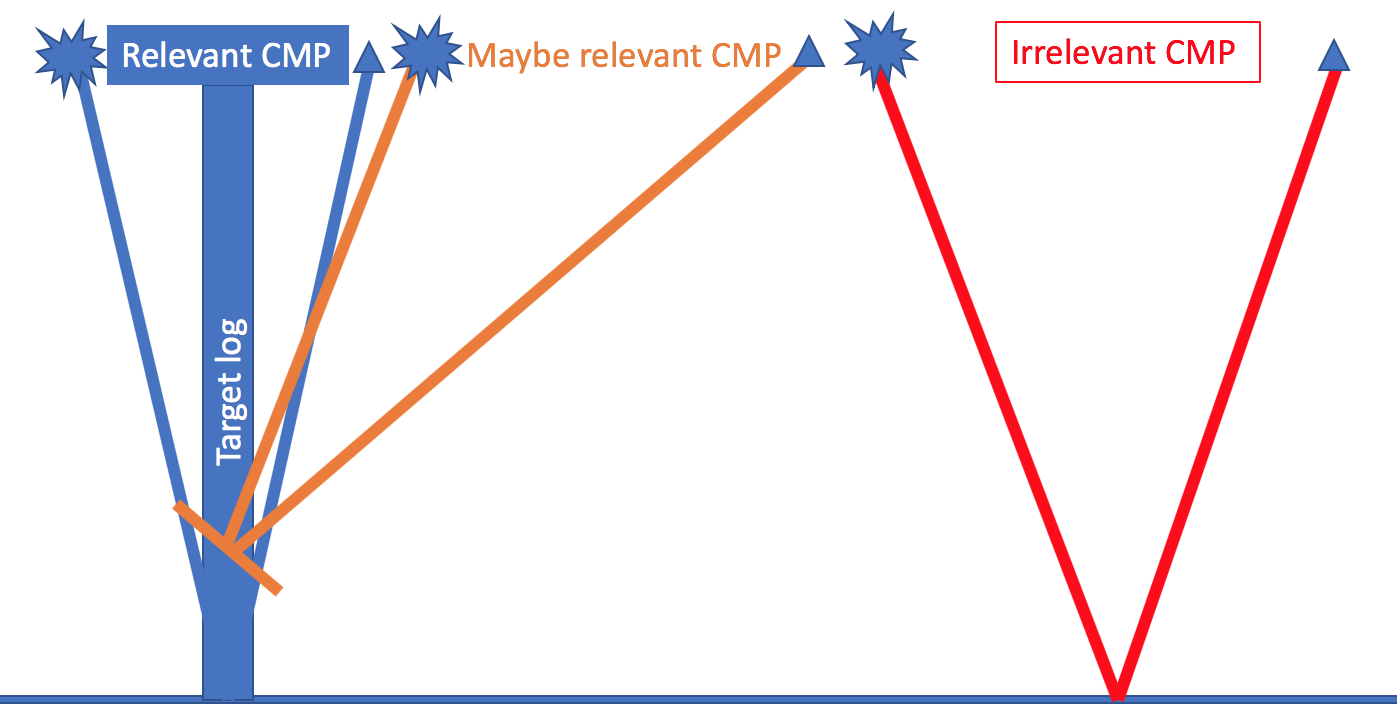
\includegraphics[width=0.7\linewidth]{Fig/relevantCMP}
	\caption{Relevant common midpoint (CMP) gathers - right above the image point location are utilized by standard stacking procedures and FWI. The gathers that are slightly shifted may also be useful in laterally heterogeneous media, but they are often ignored. CMP gathers that are far away from the imaging point are not spatially related to the imaging point, we discard those from the input}
	\label{fig:relevantCMP}
\end{figure}

Standard velocity analysis uses CMP stacking along hyperbolas to extract velocities, and then the stacked data are mapped to depth. This is good enough for horizontally layered media in most cases. More advanced velocity analysis techniques, such as common reflection surface  \citep{mann1999common} or multi-focusing \citep{gelchinsky1999multifocusing}, take care of mild horizontal velocity variations and curved reflectors relying on certain assumptions about the subsurface. We take this concept to its extreme, by relying on geologically plausible models as realistic scenarios and replacing the conventional stacking analysis with deep learning inference.

In particular, we construct a CNN that is trained to perform mapping of relevant seismic data cubes to respective velocity logs, shown in \figref{in_out}: 
\beq \label{eq:mapping}
u_{obs}(x_{CMP}-\varepsilon:x_{CMP}+\varepsilon, h_{min}:h_{max}, :) \to v(x_{CMP}, :).
\eeq
Relevant observed data $u_{obs}(x_{CMP}-\varepsilon:x_{CMP}+\varepsilon, h_{min}:h_{max}, t)$ are mapped
to an estimate of the vertical seismic velocity profile at a target location $v(x_{CMP}, z)$. Here $x_{CMP}$ is the central midpoint,
$u_{obs}$ is the observed wavefield (acoustic pressure in our case), 
$h_{min}$ and $h_{max}$ are the shortest and the longest offsets that are usable from the data, $t$ and $z$ stand for time and depth, respectively.

In the next subsection, we discuss why the mapping defined by \eqrf{mapping} is a candidate for an optimal way to cast the seismic exploration inverse problem in the deep learning set up.  
\begin{figure}[h!]
	\centering
	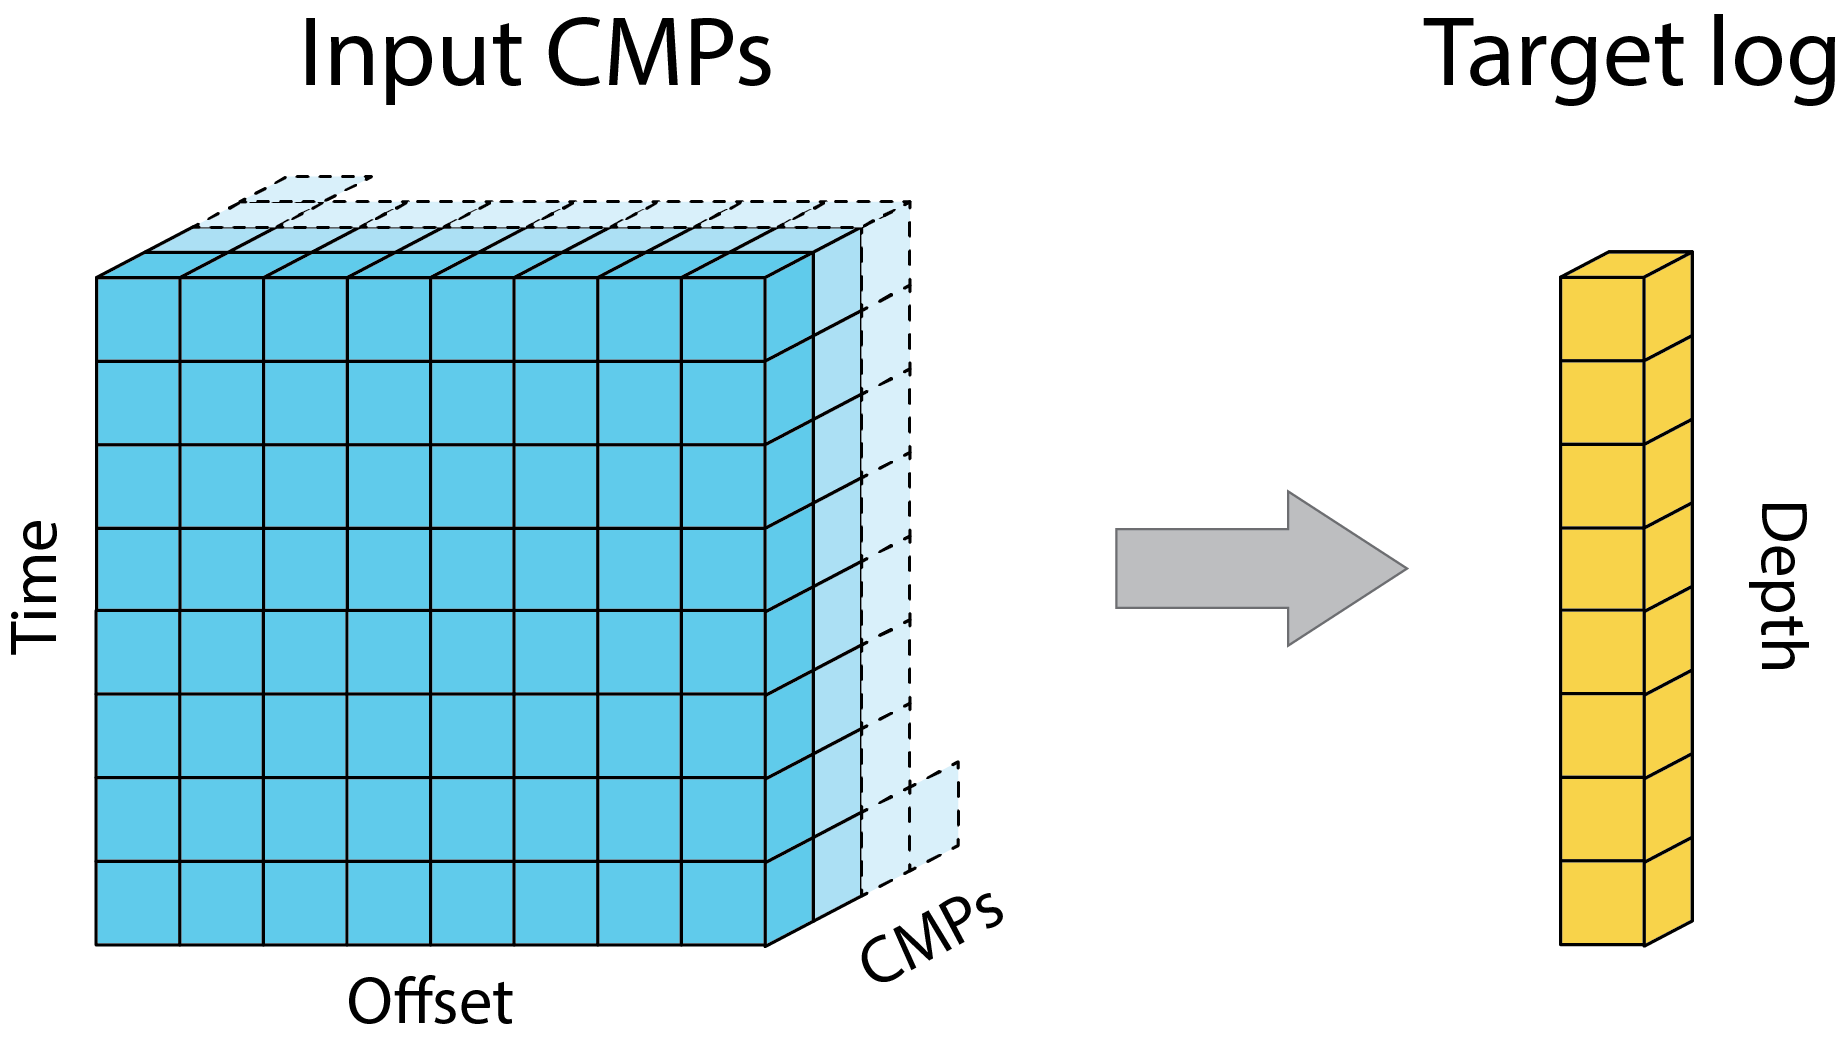
\includegraphics[width=0.7\linewidth]{Fig/in_out_shape}
	\caption{A set of neighboring CMP gathers is mapped to a velocity vertical profile with its horizontal coordinate corresponding to the middle of this set.}
	\label{fig:in_out}
\end{figure}

\subsection{Regularity of seismic data and deep learning inversion of full-waveforms}

Conventional active seismic acquisition aims at providing equal illumination to all the target areas of interest. Since the Earth's subsurface parameters are not known, we often accomplish this objective by setting up a survey that is regularly sampled in all available dimensions. Therefore the problem of vertical velocity profile estimation is exactly the same regardless of the location for a given exploration field. Taking this fact into consideration, we set up a deep learning problem that takes advantage of the similar data coverage for all locations. 

The resemblance between different locations in the field of exploration is well understood and taken into account in seismic imaging methods that rely on simplified media assumptions, such as stacking. However, it cannot be easily incorporated into methods based on full-waveform modeling such as FWI and reverse-time migration (RTM).   
%
Artificial neural networks (ANNs) can serve as universal estimators, and have no principal constraints on which data space to map. Therefore, ANNs can be utilized to infer the mapping~\eqref{eq:mapping} from data-model pairs created by full-waveform modeling. 

Finally, training deep neural networks is often computationally expensive. From the mathematical point of view mapping~\eqref{eq:mapping} is a mapping of 3D functions (5D for 3D data acquisition) on compacts to 1D functions, which should theoretically be much easier to estimate than mapping the full data to full models, which would need inference between 3D and 2D functions for 2D problems, or even in 5D to 3D for 3D problems. This makes the mapping to 1D logs an affordable and sufficient option.

%The regularity of conventional seismic exploration data and exploit the standard extended velocity analysis approach.

\section{Data}
Data-driven applications heavily depend on the quantity, features, and variability of samples in the data set, which makes data collection and selection crucial. 
%
We intend to produce virtual well logs from seismic data arranged into common-midpoint gathers. The data set for such applications should consist of input seismic data and respective target logs. However, there is a very limited amount of field samples of well logs because drilling and collection of cores is a costly task. 
%
To overcome this limitation, we generate a synthetic data set representing real-world geological features. First, we generate a set of pseudo-random subsurface models and then numerically propagate seismic waves in them. Later, recorded wavefields are assembled into CMPs and the random velocity models are decomposed into a set of well logs.

\subsection{Pseudo-random models}
Despite the clarity of intention, there is still no recognized way to generate realistic, textured all-purpose subsurface models with proper geological features.
%
Relatively realistic subsurface models could potentially be delivered by using neural networks \citep{ovcharenko2019style, wu2020building} and wavelet packets \citep{kazei2019realistically}. However, to reduce ambiguity in the model generation, multiple approaches and set ups need to be further tested.

To simplify the model generation process for the current application, we essentially combine elastic image transformations commonly used in text-recognition applications \citep{simard2003best} and cropping with stretches \citep{sunLowFrequencyExtrapolation2018} from an existing model.
%
In particular, we empirically generate pseudo-random subsurface models in three steps from the guiding model -- the Marmousi benchmark model \citep{marmousi1991}.

\begin{itemize}
%	\item First, we build the geological prior by flipping and replicating the Marmousi model (\figref{shiftsVectors}).
%	
%	\item Then, we produce a distortion map from a random Gaussian field (\figref{shiftsVectors}) and map vertical coordinates in the prior according to this field \figref{deformedModelNormal}.
%	%We then stretch coordinates further \figref{deformedModelNormal}.
%	
%	\item Finally, we crop a random rectangular patch from the deformed model and resize it back to the size of the target subsurface model (\figref{random_model_example}).

	\item First, we build a guiding geological model by flipping around the vertical axis and replicating the Marmousi model \figrefp{marm_aug}.
	
	\item Second, we crop a random rectangular patch from the deformed model and resize it back to the size of the target subsurface model (\figref{shiftsVectors}).
	
	\item Then, we produce a distortion map \figrefp{shiftsVectors} from a random Gaussian field and map vertical coordinates in the prior according to this field (\figref{deformedModelNormal}).
	
	\item Finally, we add a smooth 20\% distortion over the velocity to produce various random models \figrefp{random_model_example}.
	%We then stretch coordinates further \figref{deformedModelNormal}.
	
	
\end{itemize} 


%\dplot{stretchMarm}{stretchMarm_strip}{To generate a pseudo-random model with realistic structures we first (a) flip and replicate Marmousi. (a) Full prior model. (b) Crop of the prior with dimensions similar to the original Marmousi II model.}

%\dplot{shiftsVectors}{deformedModelNormal}{Generation of random subsurface models. Black arrows show vertical shifts (horizontal component added for better visualization) defined by random Gaussian field and applied to the geological prior -- guiding model. Guiding model before the transformation -- (a) and after the transformation -- (b). The coordinate transformation changes the order of some layers in the model, creates new layers and removes some of the other layers}
%%Random Gaussian field defines (a) vertical shifts that we apply to the model. (b) deformed model
%
%\aplot{random_model_example}{width=\columnwidth}{Five examples of generated pseudo-random model concatenated vertically}

\ffplot{marm_aug}{shiftsVectors}{deformedModelNormal}{random_model_example}{Generation of random subsurface models. (a) Guiding augmented Marmousi model. (b) Crop before the transformation. Black arrows show vertical shifts (horizontal component added for better visualization) defined by random Gaussian field. (c) Distorted model. The coordinate transformation changes the order of some layers in the model, creates new layers and removes some of the other layers. (d) Five examples of generated pseudo-random models concatenated vertically after adding a smooth gaussian field to the distorted models}
%Random Gaussian field defines (a) vertical shifts that we apply to the model. (b) deformed model


%\vspace*{-1em}
%\paragraph{Generator features}
The generator described above allows us to generate a set of models, which expand on the layered geological structure from the Marmousi model. Despite using a specific velocity reference, the generator produces a diverse range of subsurface models, which automatically satisfy the desired range of velocities. The main part of the transformation is the vertical repositioning of the local textures in the guiding model. However, depending on the smoothness of the coordinate transformation, new horizontal layers can be generated and old layers may collapse \figrefp{deformedModelNormal}.

\subsection{Seismic wave propagation}
There are no principal limitations to the type of wave equation or solver we may use. Yet, thousands of shots are necessary to generate statistically significant input for the deep learning. To reduce the computational cost of modeling, acoustic 2D \citep{polo2018,ovcharenko2018,ovcharenko2019deep, li2019} or elastic 1D \citep[e.g.][]{zheng2019} media assumptions are typically utilized. We employ acoustic modeling.

Should the model be horizontally invariant, we can try to reconstruct its elastic layers from a single shot gather \citep{roth1994} or a single CMP gather \citep{zheng2019}.
While there is limited applicability of deep learning models to laterally inhomogeneous models \citep{zheng2019}, to the best of our knowledge, training was performed on vertically variant models to speed up the data generation. Here we utilize conventional finite-difference 2D wave propagation and investigate different options for laterally variant media.
The data are generated with equidistant sources and receivers at a spacing of 100~m. We model the data with a 7~Hz Ricker wavelet and then bandpass them to 2-4 Hz. The maximum offset is limited to 4~km and the data below 2~Hz are filtered out to present a decent challenge to conventional FWI. We symmetrize the data and utilize only the positive offsets \figrefp{input_multi} based on reciprocity theory.

To generate seismic data in each random model, we integrate the Madagascar package \citep{fomel2013madagascar} into the workflow. 
We use a CUDA-accelerated acoustic finite-difference solver in the time domain to numerically simulate seismic wave propagation and to record seismograms at each receiver for every source in the acquisition.
%
% function "sfgenshots" - a cuda-based finite-difference solver. There are no principal limitations to the type of solver to be used. After that the shots are sorted into CMP gathers.

\section{Deep learning: Setup}
The general idea of deep learning is to build a mathematical model, which would derive a desired non-linear relation directly from the data. Selection of a particular deep learning model is heavily motivated by the attributes of the available data. 

%\subsection{Input and output}
%	supervised learning

\aplot{input_multi}{width=\columnwidth}{Multiple-CMP gather serving as a single input cube into the neural network in one of the training models. The CMP gather number 10 is centered on the location of the log to be estimated. The average values across CMPs at larger arrival times are close to zero, so they don't need to be zero-centered. Data at short propagation times on the other hand act more like constants -- biases. Raw data goes into the neural network.}
We map multiple-CMP gathers (\figref{input_multi}) to their respective target well logs. Both the inputs and the outputs are known arrays of real numbers; therefore, the problem reduces to a supervised task of multivariate regression.  

At the training stage, a supervised model derives a relation, which links the input and target variables for each pair in the training partition of the data set. Whereas at the inference stage, the model infers target variables when given a sample from the previously unseen test partition of the data.

Regardless of the type of deep learning models used in the application, a proper normalization is typically required for each sample of the input and target data. Normalization makes the data fit a range matching the bounds of activation functions. It also enforces more even contributions of the data features into the training. This leads to weight optimization (training) for a better convergence in a shorter time.

Seismic data are naturally centered around zero if there is sufficient variation in the data. Instead of typical data standardization, we use batch normalization as a kind of scalar scaling. After that we add random noise with 0.1 standard deviation to the input of the neural network to reduce the sensitivity of the network to low-amplitude parts of the CMP gathers. We observed that the procedure works similarly to data standardization, but allows for more robustness in the generalization of the network.

%Target data are seismic velocity profiles, those already have a range and have similar variability therefore standard Min-Max scaling to the into range $[-1, 1]$ works rather well for these data and does not change the patterns that can be extracted from those.  

The target data are seismic velocity profiles, which naturally span a narrow range of values and have similar variability. We experimented with standardization of the training data set and the common Min-Max scaling to the range $[-1, 1]$. We observed that while the Min-Max scaling leads to faster convergence on the training data set, the standardization offers better generalizability.


\subsection{Metrics}
To evaluate the quality of the trained models, we utilize two metrics on the estimated velocity $V$ based on the $L_2$ norm:
\beq
\text{NRMS}(V_{estimate}, V_{true}) \equiv \frac{100\%||V_{estimate}-V_{true}||}{||V_{true}||},~\\
\text{R2}(V_{estimate}, V_{true}) \equiv 1 - \frac{||V_{estimate}-V_{true}||^2}{||V_{true}-avg(V_{true})||^2},
\eeq
between estimate $V_{estimate}$ and ground truth $V_{true}$ velocities.
The normalized root-mean-square (NRMS) error provides a relative measure of cumulative mismatch between the predicted velocity profiles and the known target profile, with an exact match for $\text{NRMS} = 0\%$. The coefficient of determination (R2) reflects the fraction of the variance in the data that the model fits \citep{polo2018, kazei2020deep}. A model is scored higher than $0$ when its predictions are more accurate than the mean value. A perfect match is at $\text{R2} = 1$. R2 reflects the quality of the model comparable to the other models, while the mean-square-error loss is the actual optimization target.


% We empirically found that the Min-Max scaler from the Scikit-learn library \citep{scikit-learn}, applied to the set of samples shifts the mean of the seismic data away from zero as well as destroys spatial and temporal continuity in the data. Altogether this leads to the subsequent poor performance of the neural network. On the other hand, data standardization with StandardScaler (linear scaling to unit variance and zero mean) preserves continuity in the data. After the standardization, we downscale the data with an empirically chosen coefficient of 0.1 and then mute the outliers to fit all the data into the [-1, 1] range (\figref{X_scaled}).

% \dplot{X_raw}{X_scaled}{Preprocessing of input data to the network. Raw and preprocessed seismic common-midpoint gathers (a) and (b) respectively. We model the data with 7Hz Ricker wavelet and then bandpass them to 2-4 Hz. The data is then scaled by standard scaler. We utilize only positive offset as the data are synthetic and due to the reciprocity there is no difference with swapping source and receiver positions.}
%
%. We utilize only positive offset as the data are synthetic and due to the reciprocity there is no difference with swapping source and receiver positions.}


\subsection{Convolutional neural networks (CNN)}
%   spatial dependency = convolutional
Regular feed-forward neural networks, such as a multilayer perceptron, are suitable for problems with a relatively small size of input data as the number of parameters in them grows quickly with the input size. When the input volume is an image, then networks with convolutional layers come into play. Convolutional layers perform convolution of the input volume with a set of filters, which results in a set of feature maps, one corresponding to each filter. The key feature of the convolutional layer is that it admits local connectivity, which means that only a small set of neighboring points contribute to a particular point on the feature map when the filter slides over the input volume. This feature allows the network to learn spatial patterns in the data and utilize them at the inference stage.

\subsection{The architecture}
We initially considered two CNNs with exactly the same architecture apart from their first layers, which accept input data of different shapes.
%
First, we construct a 2D CNN that shifts its filters along the offset and time for individual CMPs. This neural network takes a single CMP gather as input.
The second neural network takes multiple CMPs as multiple channels in the first layer and then follows exactly the same architecture as the first neural network (shown in \figref{architecture}). 
This ``multiCMP" CNN gradually reduces the size of the input, similarly to an encoder. Every other layer replicates the previous one and reduces the size of its input twice following the same flow as in AlexNet \citep{krizhevsky2012imagenet} and VGG \citep{simonyan2014very}. The input in our case is a multi-channel image of size $(n_{offsets}, n_{timesteps}, n_{CMPs})$. Since $n_{timesteps} >> n_{offsets}$, it makes sense to consider filters that are stretched along the time axis. 

The exponential linear unit (ELU) activation function,
\beq
f(x) = max(x, \exp(-|x|) - 1),
\eeq
is applied to the output of every layer x but the last one. ELU is an upgrade to the rectified linear unit activation that improves on the dead neurons problem \citep{clevert2015fast}. The last layer of the CNN features a linear activation function. This configuration is often utilized in deep learning applications as it presents a computationally cheap way to introduce non-linearity into the network. 
Finally, we apply batch normalization after every layer in order to regularize the training process and prevent overfitting. Though \cite{clevert2015fast} observed that using ELU reduces the need for batch normalization, we observed that the weights sometimes collapse without it.
%\subsection{CNN design}

\aplot{architecture}{width=\linewidth}{Purely convolutional neural architecture allows us to easily scale the input and output data. Strides larger than one provide compression of the data within the neural network. The last layer features large convolutional filter and adjusts the output size by using valid padding.}


\section{DL: Training}
Fitting within the CNN happens through the optimization of multiple filters. First, the CNN filters are initialized with random values, and then those are optimized to match the output. The optimization is typically executed with a local search method through backpropagation of errors of the neural network on training data set. We use one of the popular optimization algorithms, Nadam \citep{dozat2016incorporating}, which is an adaptive moment estimation (Adam) enhanced by the Nesterov accelerated momentum.

%The network is trained given the training part of the data set whereas its performance is estimated by evaluation of inference result on the validation data. Final performance is measured from inference on testing data.

%\subsection{Standard data splitting}
% Why commented below?
%


%We extract the last 10\% of samples and split them into 5\% for testing and 5\% that are always used in training that we perform throughout the paper. These 10\% of the data we later on utilize to visually inspect the fitting for training and testing samples. The rest, 90\% of the data are split according to Pareto principle \citep{dunford2014pareto} into training and validation sets randomly (\figref{T_data_split}).
%We split data set into  

\subsection{Standard training}

The classic deep learning process starts with splitting all available data into training, validation and testing subsets. 
The goal of training is
%not learning the input-output relation as a data base or dictionary, but 
to infer the dependence between the input and the target data such that it can further be applied to other data. Therefore, the performance of the CNN is evaluated throughout the process of training by applying the neural network to validation data. Once the CNN stops improving its performance on the validation data set, the training stops. The validation data is utilized for monitoring the training process and should not be used to evaluate the model performance. Thus, a small portion of the whole data is isolated from the training procedure to form the test data set. 

Often the three subsets of the data are determined randomly. However, it is not fair in our case, since the samples are spatially correlated. If the CNN sees neighboring logs in the training, all it would learn would be the simple interpolation between them. To mitigate this problem when testing the neural network performance and in order to examine its performance on training samples, we split the data set in the following way: 77\% for training, 18\% for validation and 5\% for testing. The total number of models generated is 1,000; we observe that using 50 of them is relatively stable for testing.

Once the training set is organized, we need to choose the optimization strategy. This typically includes an optimization algorithm and its parameters. We empirically find that a batch size of 64 provides high yet stable performance over epochs in our case for about 57,000 samples. Nadam provides a rapid decrease in the loss function. We notice that the validation loss essentially stops decaying after about 20 epochs for both neural networks. Then the learning rate is decreased to further fit the data. Both CNNs tend to overfit the data, which to some extent is prevented by batch normalization and by early stopping on condition of no validation loss decay over 7 epochs. Training takes about 60 sec per epoch for the single-CMP neural network, and about 120 sec per epoch for the multiCMP CNN. Both networks are trained on a single RTX Quadro 8000 GPU. Neither network gains any performance by moving to a multi-GPU data-parallel training; we associate this with the relatively small batch size and poor parallelizability of the batch normalization layers. Also, the multiCMP CNN has a larger number of input channels/data per sample; thus, the throughput of the samples provides an additional constraint on the parallelization. From the classic training procedure, we compiled Table~1,~which~suggests~significant~overfitting~in~the~learning~process.

As expected from physics of wave propagation in laterally heterogeneous media, the multiCMP CNN is more suitable for inversion. Namely, the ratio of NRMS error on training and testing data is higher and, most importantly, the NRMS error is lower for the validation data set. We therefore discard the single-CMP neural network from further analysis. We also tested including a wider range of CMPs into multiple-CMP gathers, which we then used as individual training samples. There was no gain in performance of the network on this particular data set, so we fixed the architecture for further analysis.
%
\subsection{}
\begin{table}
    \begin{center}
	\begin{tabular}{||c | c | c ||}
		\hline
		Filter size & single-CMP train/\textbf{test} NRMS & multiple-CMP train/\textbf{test} NRMS \\ \hline\hline
		(3, 3)    & 4.2/10.4                   & 2.3/9.3                  \\ \hline
		(3, 7)    & 2.3/9.1                   & 1.3/7.3                  \\ \hline
		(3, 11)   & 1.7/8.9                   & 1.3/\textbf{\underline{7.1}}        \\ \hline
		(3, 15)   & 1.4/\textbf{8.5}          & 1.1/7.2                  \\ \hline
	\end{tabular}
	\caption{The validation and training quality depending on the filter size. The multiCMP CNN performs best on the test data set with a filter size of 3 samples in offset and 11 samples in time.}
	\end{center}
\end{table}
%

\subsection{Dynamic learning}
The standard practice of learning with static data sets suffers from overfitting. To overcome the issue, data augmentations are typically introduced. We add random Gaussian noise to the outputs of all the layers except the last one, which could be considered the most generic data augmentation. More interestingly, the process of generating the data set could be considered as an augmentation itself. We therefore develop the following approach: 100 models are generated and the respective data samples are loaded as the static validation data set. The training data set, on the other hand, is considered dynamic. We generate 100 random models in the training process and model the data. When the new data are ready, they are fed into the CNN. Thus, new models and data are generated asynchronously with training. We observe that generation of the data related to 100 random models with 3 GPUs takes about 90 sec. Training the neural network for a single epoch takes about 60 sec. Therefore, if we distribute data generation to 3 GPUs and train the model on the left one, we can keep training the network at the same speed. About every 1.5 epoch, we replace the training data. This way, the training data set is effectively infinite and the overfitting is reduced. We sequentially train an ensemble of five multiCMP neural networks and observe gradual reduction in the overfitting \figrefp{multiCMP_loss_Full}.


%\fplot{T_data_split}{train_single-CMP_predicted}
%{train_multiCMP_predicted}{train_multiCMP_true}{(a) Training set is split into: training, testing and validation parts. (b) Last 10\% of the data set. First 5\% are used in training and the last 5\% are not. (c) and (d) Predicted velocity logs by single CMP data and from multi CMP data.}

\subsection{Reproducibility}
One of the main features of the neural networks is their stochasticity. There are multiple reasonable mappings that the neural network could learn in a multidimensional regression setting. Leaving the randomness of our training data set out of scope (we fix the seed for reproducibility of the data set), stochasticity of the neural networks comes from several factors: random weight initiation, random training set shuffling, and random parallel arithmetic operations order inside the GPU. While the first two factors could in principle be isolated by random seed selection, the third one is very hard to deal with. Apart from that, particular choices of random initial weights should not significantly affect the inversion results.

Therefore, instead of going for exact numerical reproducibility, we try to provide a clue about the randomness of our estimates by training multiple instances of our neural networks on the same data set. In order to keep the computational time within a few hours, we take only five instances of each network, which is not enough to get a reasonable uncertainty estimate but it can provide us with some insights into it. In the next section, we test our trained ensemble of five CNNs. Note that flipping the input along the CMP axis should not change the output, yet it effectively leads to coupled CNNs. We can, therefore, increase the ensemble to 10 different estimates.

\dplot{multiCMP_loss}{multiCMP_R2}{Evolution of (a) the loss functions and (b) the coefficients of determination on training and validation data sets. The thicker line indicates the model with lowest final validation loss. Despite the use of different data sets for training of each of the models their metrics are very close.}

\section{DL: tests on other models}
In most deep learning applications to seismic inverse problems, the models are significantly simplified. Here we go for the full model complexity. The section consists of three subsections. First we examine the performance of the ensemble of five multiCMP CNNs on the Marmousi II model, which is very similar to the guiding Marmousi model utilized for the training data set generation. 
%
% We start with a pseudo-1D model generated by a horizontal stretching of the guiding model, then by random deformation of that model, which is still for the most part horizontally layered. After that, we apply our inversion to the guiding Marmousi model itself. 
%
Then we examine an application to two rescaled crops from the SEAM Phase I model \citep{fehler2011seam}. Finally we show an application on the Overthrust model of the multiCMP CNNs and subsequent FWI. For each example, we compute the average and the standard deviation of the outputs within the ensemble.

%% figure naming convention:
%(train/test)_(prefix(single-CMP/multiCMP))_{folder(for train: ""=x1,x2,x3:marmvel1D, marmvel1D_distort,marmvel,overthrust1D,overthrust2D)}_{inverted/true/X_scaled}

% \subsection{Guiding model and its derivatives}

% Despite the diversity of pseudo-random subsurface models used for training, these are still biased toward the guiding model which has been selected as prior. The purpose of this section is to investigate the behavior of the deep learning model when applied to different scenarios derived from the original guiding model.

% \paragraph{Marmousi 1D}
% \newcommand{\modelFname}{marmvel1D}

% The first question that we would like to answer is if the CNN that we trained can fit part of the stretched Marmousi model (\figref{\tm\modelFname_true}), yet was not used in training directly. \figref{\tm\modelFname_true_Full} shows the results of inversion for synthetic data acquired in such a model. Data in this case are not significantly clipped (\figref{\tm\modelFname_X_scaled}) and do not vary significantly between multiCMP input channels. The input of multiCMP CNN is largely redundant as the model is essentially 1D. Therefore as expected CNN utilizing single CMP input is performing better (\figref) than the multiCMP CNN (\figref{\tm\modelFname_inverted}). This fact is also reflected in the standard deviation maps (\figref{test_single-CMP_\modelFname_inverted_std_dev} and \figref{\tm\modelFname_inverted_std_dev}). Standard deviation maps describe inconsistency between log estimations by five identical but independent networks. These were trained by starting from different weight initializations and thus converged to slightly distinct final results. The ensemble of CNNs is obviously not sufficient to estimate variance properly, yet we notice that the variance is increasing with depth and is focused around the deeper high-velocity layer location.


% \fplot{\tm\modelFname_true}{\tm\modelFname_X_scaled}{\tm\modelFname_inverted}{\tm\modelFname_inverted_std_dev}
% {(a)Test model -- stretched crop from the left edge of the Marmousi model. (b) Rescaled CMP gathers used as the first and the last channels of an input sample of multiCMP CNN. Average estimate from the ensemble of (b) -- single-CMP CNNs and (c) -- multiCMP CNN. Standard deviation for the (d) -- single CMP CNN outputs, (e) -- multiCMP CNN outputs. }

%\paragraph{Distorted Marmousi 1D}
%\renewcommand{\modelFname}{marmvel1D_distort}
%The second question is if the trained CNN would fit another model generated from Marmousi 1D by an elastic transform. While the guiding model is for the most part horizontally layered, large coordinate shifts create lateral variations (\figref{\tm\modelFname_true}). We notice that shallow laterally varying anomalies can to some extent be estimated by both CNNs (\figref and \figref{\tm\modelFname_inverted}). Standard deviations within ensembles (\figref{test_single-CMP_\modelFname_inverted_std_dev} and \figref{\tm\modelFname_inverted_std_dev}) suggest that the deeper part is not very well resolved by both CNNs. The shallow parts of the model are resolved rather well and the largest uncertainty is focused at the interfaces of shallow anomaly in the left part of the test model. Data representative in this case is not clipped much and shows visible amplitude variation between multiCMP channels (\figref{\tm\modelFname_X_scaled}).

%\fplot{\tm\modelFname_true}{\tm\modelFname_X_scaled}
%{\tm\modelFname_inverted}
%{test_single-CMP_\modelFname_inverted_std_dev} {\tm\modelFname_inverted_std_dev}
%{Same as \figref{\tmmarmvel1D_true_Full}, but for distorted 1D profile from Marmousi model. (e) The lateral heterogeneity becomes obvious in the CMP gathers}


%\paragraph{Original Marmousi}
%\renewcommand{\modelFname}{marmvel}
%Guiding model -- Marmousi (\figref{\tm\modelFname_true}) was not directly added to the training set, but was used for the training set generation. It is largerly laterally heterogeneous, yet single CMP CNN provides a reasonable estimate (\figref), which would probably be good enough for a subsequent FWI application. On the other hand some layers introduced into the inversion result by single-CMP CNN are artificial. We attribute it to the limited information contained in single-CMP data. multiCMP CNN corrects for the artifacts (\figref{\tm\modelFname_inverted}). The standard deviation maps (\figref{test_single-CMP_\modelFname_inverted_std_dev} and \figref{\tm\modelFname_inverted_std_dev}) suggest that multiCMP neural network provides a better estimate in this case. In the shallow part of the model the multiCMP CNN standard deviation (\figref{test_single-CMP_\modelFname_inverted_std_dev}) has lower amplitude. In the deeper part of the model, it is more focused around the interfaces.  
%
%\fplot{\tm\modelFname_true}{\tm\modelFname_X_scaled}
%{\tm\modelFname_inverted}{\tm\modelFname_inverted_std_dev}
%{Same as \figref{}, but for the Marmousi model itself}

%The properly trained neural network should exhibit generalization capability. Meaning that it should infer meaningful result when applied to unseen data. However, when the new input data is sufficiently different from the training data, the estimate is expected to be inaccurate. In this paragraph, we demonstrate three applications of the network to the data significantly different from the one in training data set. The first application is for salt-induced SEAM Phase I model, which produces data with strong reflections inconsistent with CMPs produced by a non-contrast training data. Other two examples are for 1D and 2D Overthrust models which resemble the layered structure of subsurface models used for training, however with different contrasts and layer inclination.

\subsection{Marmousi II}
\renewcommand{\tm}{test_multiCMP_}
\newcommand{\modelFname}{marm2}
Marmousi II model (\cite{martin2006marmousi2}, \figref{\tm\modelFname_true}) is an updated version of the guiding Marmousi model (\cite{marmousi1991}, \figref{marm_aug}). The data generated in this model \figrefp{\tm\modelFname_X_scaled} are similar to the training data set. This leads to a decent inference of subsurface parameters by the trained network. In the shallow part of the model, the multiCMP CNN retrieves a low-velocity anomaly \figrefp{\tm\modelFname_inverted} that is not present in the Marmousi model. In the deeper part, fine layering is not recovered. 
%The general observation is that the network performance is superior for portions of well logs with sparser distributions of the interfaces. This is mostly notable in the central part of the Marmousi model where the network fails to recover the fine layering in the bottom of the model while succeeds in highlighting the more shallow high-velocity layers surrounded by low-velocity sedimentary environment.
Standard deviation maps
describe inconsistency between the velocity estimates from the five independently trained CNNs.
These were trained by starting from different weight initializations and with different pseudo-random model sets, and converged to slightly distinct final results. The number of ensemble members is obviously not sufficient to estimate
variance properly, yet we notice that the variance increases with depth and is focused
around the deeper high-velocity layer location \figrefp{\tm\modelFname_inverted_std_dev}. Also, it suggests that the deeper part of the model under the strong reflectors is poorly resolved. High-velocity salt intrusions contribute the most into the mismatch distribution. Large contrast interfaces are quite often associated with larger uncertainty as minor shifts in the interfaces lead to significant changes in the velocity \citep[e.g.][]{galetti2015uncertainty}. 
%The reason is the standard deviation is measured in absolute values while metric the normalized by the respective mean value leads to more homogeneous error distribution. \todo{What do you think?}

\fplot{\tm\modelFname_true}{\tm\modelFname_X_scaled}{\tm\modelFname_inverted}{\tm\modelFname_inverted_std_dev}{(a)Test model -- the Marmousi II model. (b) CMP gathers used as the first and the last channels of an input sample of multiCMP CNN. Average estimate from the ensemble of (c) -- multiCMP CNN. The low-velocity anomaly in the top right corner is retrieved. (d) Standard deviation for the ensemble outputs.}

\subsection{SEAM Phase I}
The SEAM Phase I model exhibits sedimentary layering with large embedded salt formations. The depth of the model is much larger than 3~km; therefore, we need to either rescale the model or crop a chunk of it. We consider two geological cases extracted from the same benchmark model. First, we apply the ensemble of CNNs on a crop with sedimentary layering. Second, we examine the network capability on a rescaled section with a salt body.

\subsubsection{SEAM I. Layering without salt}
\renewcommand{\modelFname}{seam_i_sediments}
We crop a chunk of the sediments from the SEAM Phase I model next to the ocean bottom \figrefp{\tm\modelFname_true}. The model is layered with increasing velocity with depth, so FWI-like methods are likely to succeed. We model the data there \figrefp{\tm\modelFname_X_scaled} as if we had redatumed the data from airguns to the ocean-bottom data. Therefore, we don't take into account the wave propagation through the upper water layer. 
% The multiCMP estimate of the velocity is nearly indistinguishable from the true model.
The multiCMP estimate of the velocity results in a smooth model that is nearly indistinguishable from the true model \figrefp{\tm\modelFname_inverted}. However, the standard deviation map suggests that there is an increase in the variability of the estimates at depth \figrefp{\tm\modelFname_inverted_std_dev}. This means that the resulting subsurface model is likely to be sufficient for conventional imaging, but might need to be updated for time-lapse FWI, in which small perturbations matter.

% It is worth mentioning that the network is trained exclusively on an augmented data set built from the Marmousi model. 
% \figrefp{\tm\modelFname_inverted}. However the standard deviation map suggest that there is some increase in the variability of the estimates at depth \figrefp{\tm\modelFname_inverted_std_dev}. The latter means that the model is probably good enough for conventional imaging, but might need to be updated if utilized for time-lapse FWI or similar procedure where small perturbations matter.


\fplot{\tm\modelFname_true}{\tm\modelFname_X_scaled}{\tm\modelFname_inverted}{\tm\modelFname_inverted_std_dev}{Same as \figref{test_multiCMP_marm2_true_Full}, but for a crop from the SEAM model. (b) The CMP gathers at 2~km apart look very similar and resemble some of the training data. (c) Nearly perfect reconstruction of the model is supported by low standard deviation (d).}

\subsubsection{SEAM I. Salt body}
\renewcommand{\modelFname}{seam100}
The salt-affected part of the SEAM Phase I model features strong reflections from the salt flanks. This type of event is poorly represented by the CMPs in the training data (\figref{\tm\modelFname_X_scaled}). On the other hand, the inversion recovers the velocity trends next to the salt and the salt boundary \figrefp{test_multiCMP_\modelFname_inverted}. The CNNs were not given a sufficient amount of data/models featuring salt bodies. Therefore, they are more likely to produce layers rather than large homogeneous high-velocity objects. 
The central part of the deviation map inside the actual salt position dominates over the neighboring regions. This could be utilized to potentially find the areas that are not properly inverted and alter them with model interpolation, similarly to variance-based model interpolation for conventional FWI \citep{ovcharenko2018}. Both the sedimentary sections on the sides of the salt body and the top of the salt body are retrieved; therefore, the estimated model could also be useful for salt flooding and subsequent FWI \citep{kalita2019regularized}.

\fplot{\tm\modelFname_true}{\tm\modelFname_X_scaled}{\tm\modelFname_inverted}{\tm\modelFname_inverted_std_dev}{Same as \figref{test_multiCMP_marm2_true_Full}, but for the rescaled crop from the SEAM model. (b) Events around the 6 sec in the right CMP gather. Standard deviation shows that the top part is reliable, but otherwise is not correlated with error in the estimate in this case.}





%We split the phenomena into two. First, we replicate low-relief part of the Overthrust model to test the layer stripping capabilities of the trained CNNs and then we test on the full model extended by replication and flipping.

% \subparagraph{Overthrust 1D}
% \renewcommand{\modelFname}{overthrust1D}

% Shallower layers in this model feature low contrasts and velocity increases and then decreases (\figref{\tm\modelFname_true}). The data \figref{\tm\modelFname_X_scaled} scaling shows very strong first arrivals and very low amplitude reflections, which focuses inversion on the near-surface anomalies.
% Both CNNs seem to get the top of the model right (\figref,
% \figref{\tm\modelFname_inverted}) and fail at the bottom part. Single CMP CNN fails in a bit more moderate way as expected for this low-relief model. Deeper layers are mispositioned, which is reflected in overall increasing standard deviations within the ensembles (\figref{test_single-CMP_\modelFname_inverted_std_dev} and
% \figref{\tm\modelFname_inverted_std_dev}). 

% \fplot{\tm\modelFname_true}{\tm\modelFname_X_scaled}
% {\tm\modelFname_inverted}{\tm\modelFname_inverted_std_dev}
% {Same as \figref{\tmmarmvel1D_true_Full}, but for the pseudo-1D model generated from Overthrust model}

\subsection{Overthrust 2D (DL + FWI)}
In order to further explore the generalization power of the trained CNNs, we test them on data modeled in a slice of the Overthrust model (\figref{true_overthrust}). This model is challenging for FWI due to its low-velocity layers, which are squeezed between high-velocity reflectors. It is also challenging for conventional layer stripping due to the presence of uplifts and faults. The CNNs recover most of the large scale features of the model. For the most difficult to resolve part of the model (near faults), the deep learning (DL) estimate is not perfect \figrefp{dl_overthrust}. In order to improve the model estimate in that region, we run FWI of the full-band data with the source central frequency of 7~Hz. After 75 iterations of the preconditioned conjugate gradient optimization of full-band, full-offset data, the predicted model is improved \figrefp{fwi_overthrust}. Each iteration of FWI takes about 4.5 sec.

We compare the 1D vertical velocity profiles estimated by the CNNs (DL), updated by FWI (DL + FWI) and the ground truth profiles at 6, 12, and 18~km positions. The simple part of the model, at 6~km, is estimated well by all methods \figrefp{log_6}, with some refinement gained from FWI in the deeper part. At the more complicated 10~km position, the DL estimate is good for the shallower reflector at 1~km and then degrades in the poorly illuminated zone \figrefp{log_10}. At the 12~km position, the estimate suffers from significant underfit in the mid-depth region. In all the cases, the general low-wavenumber trend of the model is captured and improved upon by FWI. Further iterations of FWI would probably lead to an even better model estimate.
\renewcommand{\modelFname}{overthrust_test_2D_2}

\ssplot{true_overthrust}{dl_overthrust}{fwi_overthrust}{log_6}{log_10}{log_12}{(a) FWI result. Velocity logs estimated by DL and DL + FWI, compared to the true velocity model at (b) 6~km, (c) 10~km, and (d) 12~km positions.}  

Standard deviation \figrefp{\tm\modelFname_inverted_std_dev} of the multiCMP estimates correlates well with the errors in the predicted logs. At the 6 and 12~km positions, the deviation is relatively low. While at 10~km, we see a larger deviation.
The data \figref{\tm\modelFname_X_scaled} shows very strong first arrivals and very strong late reflections. Those reflections are most likely multiples and, therefore, it is hard to train CNNs to position those properly.

\dplot{\tm\modelFname_inverted_std_dev}{\tm\modelFname_X_scaled}{(a) Standard deviation of the multiCMP estimates correlates well with the errors in predictions visible in the logs. At 6 and 12~km positions the deviation is relatively low. At 10 km we see a larger value in the deviation. (b) Single input sample for the left, flat part of the Overthrust model.}

%From the last test we clearly see a rather obvious fact -- single CMP gather cannot be mapped into velocity log successfully without the assumption of laterally slowly variant medium. We believe that this is a good motivation to study the mapping of multiple CMP gathers.

\subsection{Computations: DL vs FWI}

The efforts put into general training result in an ensemble of CNNs that can be directly and instantly utilized on different data sets. The application of trained CNNs presented here takes less than 1~ms for inference per sample (CMP gather). Conventional FWI takes 10-300 iterations. Each iteration of conventional FWI requires at least two modeling runs for each shot. The training of the network for one epoch on a single GPU takes less time than generating a single data chunk on three GPUs. Training is at least twice slower than inference. Therefore, we can expect the inference with a trained network to be at the very least 10*2*2 = 40 times faster than conventional FWI. In our particular application, FWI took approximately 4.5*75~sec~$\simeq$~5~minutes on a single GPU, and the inference happens in less than 1 sec. On the other hand, training of a single CNN takes about two hours, which is equivalent to about 25 FWI applications. Training the whole ensemble of five CNNs is computationally similar to 125 FWI applications. These comparisons are heavily dependent on the implementation and are more of a guideline than a strict comparison of the computational efficiency of the methods.

\section{Discussion}

For regularly sampled seismic data acquisition, which is typical in seismic exploration, the problem of full-waveform-based velocity-model building can be reduced to the search for mapping from 3D data (relevant traces) to 1D data (single velocity logs). This formulation is not a viable option for conventional FWI implementations because the velocity model needs to be optimized as a whole. Deep neural networks, on the other hand, are universal estimators and can be trained to map arbitrary input to target data samples as long as there is such a mapping. Therefore, training for the inference of particular velocity logs from data sets is a viable option for deep-learning-based velocity-model inference.

For a DL application, it is beneficial to split the whole data set into relevant and irrelevant data to speed up training. Therefore, we extracted the data (CMP gathers) from the neighboring area to the target vertical velocity profile location. 
We seek to infer the non-linear relations between the raw seismic data, arranged into CMP gathers, and the respective velocity profiles by using artificial neural network. In particular, we constructed two CNNs for this purpose and analyzed their capabilities.
% We tried to infer this relation between these data and the respective velocity logs by using CNNs. 
% In particular, we constructed two CNNs to infer this relation between the data and the vertical velocity profiles and analyzed their capabilities.
The first CNN accepts the single-CMP data as input, and the second CNN accepts multiple neighboring CMP gathers as input. We trained both neural networks on data modeled in augmentations of the Marmousi model, produced by elastic deformations and cropping. The multiCMP CNN had a better learning capacity and performed better on models with significant lateral variations. For this reason, throughout the study we focused on multiCMP CNN applications. 
% Both CNNs failed to construct a salt body, which suggests that the augmentations of the Marmousi model lead to limited capacity for generalization. So far we suggest that the same CNNs can be applied for similar exploration scenarios. The training data set must be extended further to accommodate models that are geologically very different from the guiding model. 

% \todo{Discuss application to a general model following editor's suggestion}

An ideal general-purpose neural network should produce plausible results when applied to an arbitrary data set. Obviously, building such a model is a non-trivial task that requires advances both from algorithmic and training data sides. For the multiCMP CNNs presented here, low relief structures are the easiest target. Salt bodies cannot yet be inverted, though inclined reflecting layers can be recovered.

In the described DL approach, the velocity models are built automatically from raw recorded waveforms. The resolution of these models is comparable to that of traveltime tomographic models rather than FWI models. However, the models built here are useful as starting models for FWI. Trained neural networks could provide an ensemble of starting models for an FWI uncertainty analysis.

% The multiCMP CNN is trained on a large variety of data, therefore it can potentially succeed on a general data set. Perhaps the main feature of the guiding model: large number of layers and dominance of the vertical variations over the horizontal determines optimally suited for application scenarios. Low relief structures are an easy target for the network, yet with the presence of distorted layers (like in the Overthrust model) the network performs well too. The ensemble presented here was trained on the limited offset data without very low frequencies. It is well-known that FWI performs much better when such data are available. We, therefore, can expect similar behavior from the trained networks.

% \todo{Discuss application to a general model following editor's suggestion}

% The application of trained CNNs presented here takes less than 1ms per sample (CMP gather). Therefore, with these CNNs, velocity models can be built much faster than they are currently built. The velocity models would also be built automatically from raw recorded waveforms. The resolution of the built models is comparable to traveltime tomographic models rather than FWI models. However, the models built in this way be useful as starting models for FWI. Several instances of trained neural networks naturally provide an ensemble of starting models for the FWI uncertainty analysis.

% \todo{put this somewhere?}
% FWI is a local optimization technique, while the trained ensemble of CNNs is not constrained to particular application. This leads to much larger efforts in exploring the space of possible models while training of the network. On the other hand the efforts result into trained ensemble of the networks can be directly and instantly utilized on a different data set (with questionable outcome but fast).



\section{Open-access data}
\vspace*{-0.5\baselineskip}
We relied on open-source package Madagascar \citep{madagascar} for modeling and manipulations on regularly sampled seismic data.
Machine learning implementation is based on Keras \citep{chollet2015keras} and TensorFlow \citep{tensorflow2015-whitepaper} frameworks.
\\
Additional reproducible examples are available at
\href{https://github.com/vkazei/deeplogs}{https://github.com/vkazei/deeplogs}.

\section{Conclusion}

Deep learning allowed us to estimate the mapping between raw seismic data (multiple-CMP gathers) and vertical velocity profiles. This mapping is represented by trained purely convolutional neural networks (CNNs). Namely, we trained CNNs to map the relevant data cubes to 1D velocity profiles, rather than full velocity models. This is a key feature of our method that reduces the complexity of the training process and opens an opportunity for direct usage of the sonic logs for velocity-model building with deep learning.
 
Just like FWI, our method relies on full-waveform modeling and utilizes all available data. Therefore, there are no principal limitations to the complexity of models that can be inverted. Just like in FWI, some prior assumptions about the velocity model are necessary to mitigate non-uniqueness in the seismic inversion. These assumptions can easily be incorporated into the training set. Every application of conventional FWI requires numerous forward problem solutions in order to perform the model optimization. Once the network is trained on a data set, other data sets with similar acquisition parameters and geological features can be inverted much faster than with conventional FWI. If necessary, the quality of the estimated model can also be subsequently improved by FWI.



%Therefore, if a neural network is trained on sufficiently representative of the geologic region set of models it can potentially replace other full-waveform based velocity model building methods. bringing us one step closer to real-time velocity model building with uncertainty quantification.




%The mapping in the form of a trained CNN allows us to build velocity models directly from surface seismic data.


 
%We constructed and trained two purely convolutional CNNs that map the relevant data to 1D vertical velocity profiles. multiCMP CNN has better capabilities to learn complex models, while single-CMP CNN works better for velocity models with mild velocity variations. 




%Training of neural networks is a computationally intensive process. 
%


\section{ACKNOWLEDGMENTS}

We thank the editors of Geophysics, two anonymous reviewers and Jan Walda from the University of Hamburg for their comments and suggestions that improved the manuscript.  
We also thank Adam Grzywaczewski of NVIDIA, Anatoly Baumstein and Husseyin Denli of ExxonMobil, members of the Seismic Modeling and Inversion group (SMI) and the Seismic Wave Analysis Group (SWAG) at KAUST for constructive discussions on deep learning. We are grateful to Saudi Aramco for support.
The research reported in this publication was supported by funding from King Abdullah University of Science and Technology (KAUST), Thuwal, 23955-6900, Saudi Arabia.

%\newpage
%\figref{learningParadigm} shows a speculative comparison of different seismic model building tools.
%
%\begin{figure}
%	\centering
%	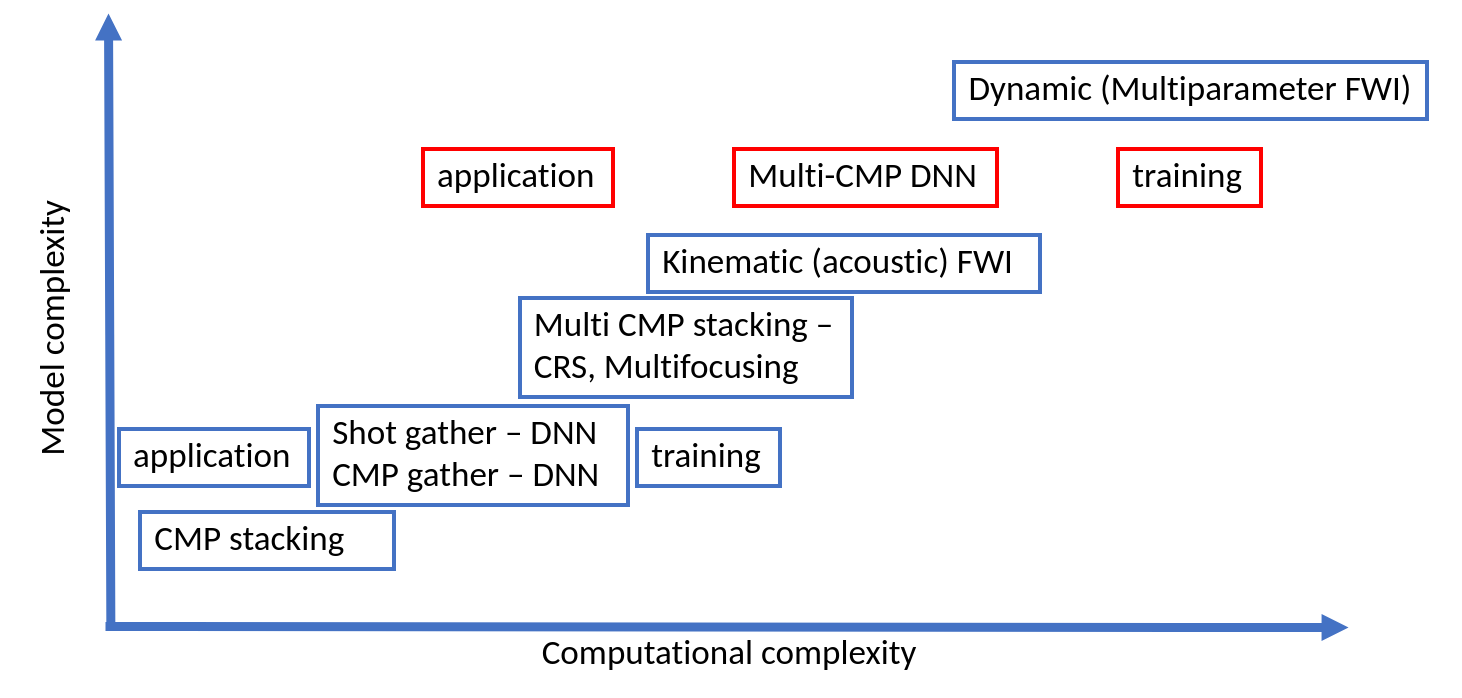
\includegraphics[width=0.9\linewidth]{Fig/learningParadigm}
%	\caption{Deep learning is rather intensive in the training part, however the application of the trained deep neural network (DNN) is nearly instant }
%	\label{fig:learningParadigm}
%\end{figure}


%\append{Selection of the filter size for the network}


\bibliographystyle{apalike}  % style file is seg.bst
\bibliography{zotero}

\end{document}